%! TEX program = xelatex
%! TEX root = ../main.tex
%! TEX encoding = utf-8

%%%%%%%%%%%%%%%%%%%%%%%%%%%%%%%%%%%%%%%%%%%%%%%%%%%%%%%%%%%%%%%%%%%%%%
%
%  哈尔滨工程大学学位论文 XeLaTeX 模版 —— 正文文件 chap04.tex
%
%  版本:1.0.0
%  最后更新:
%  修改者:Leo LiWenhui lwh@hrbeu.edu.cn
%  修订者:
%  编译环境1:Ubuntu 12.04 + TeXLive 2013/2014
%  编译环境2:Windows 7/8  + TeXLive 2013/2014
%
%%%%%%%%%%%%%%%%%%%%%%%%%%%%%%%%%%%%%%%%%%%%%%%%%%%%%%%%%%%%%%%%%%%%%

\chapter{插图}[Figure]
\label{chap05}

\section{研究生院的插图规范}[Requirement of Figure]
图应有自明性。插图应与文字紧密配合,文图相符,内容正确。选图要力求精练,插图、照片应完整清晰。图中文字和数字等字号用宋体~5~号字。

机械工程图:采用第一角投影法,严格按照~GB4457---GB131-83《机械制图》标准规定。

数据流程图、程序流程图、系统流程图等按~GB1526-89~标准规定。

电气图:图形符号、文字符号等应符合附录~3~所列有关标准的规定。

流程图:必须采用结构化程序并正确运用流程框图。

对无规定符号的图形应采用该行业的常用画法。

坐标图的坐标线均用细实线,粗细不得超过图中曲线,有数字标注的坐标图,必须注明坐标单位。

照片图要求主题和主要显示部分的轮廓鲜明,便于制版。如用放大或缩小的复制品,必须清晰,反差适中。照片上应有表示目的物尺寸的标度。

引用文献图表必须标注出处。


\subsection{图题及图中说明}[Note of Figure]
每个图均应有图题(由图序和图名组成),图名在图序之后空一格排写。图序按章编排,如第~1~章第一个插图的图号为“图~1.1”等。
图题置于图下,硕士论文可只用中文书写,博士论文用中、英文两种文字居中书写,中文在上,要求中文用宋体~5~号字,英文用~Times New Roman 5~号字。有图注或其它说明时应置于图题之上。引用图应注明出处,在图题右上角加引用文献号。
图中若有分图时,分图题置于分图之下或图题之下,分图号用~(a)、(b)等表示。

图中各部分说明应采用中文(引用的外文图除外)或数字项号,各项文字说明置于图题之上(有分图题者,置于分图题之上)。

\subsection{插图编排}[Arrangment of Figure]

插图之前,文中必须有关于本插图的提示,如“见图~1.1”、“如图~1.1~所示”等。插图与其图题为一个整体,不得拆开排写于两页。
插图处的该页空白不够排写该图整体时,则可将其后文字部分提前排写,将图移到次页。

\section{LaTeX~中推荐使用的图片格式}[Figure Foramt]

论文使用的图片都放在figure文件夹中,图片可以是~EPS、JPG、PDF等格式。插图浮动环境是\texttt{figure},基本命
令是\texttt{includegraphics},而在图片环境中,标题的位置必须位于图片的下方。

\section{单张图片}[Single Figure]

单张图片示例如图\ref{fig:wedding}所示。插入方法为插入浮动图后,在图片位置插入所需图片。一般需要使用段落设置将图形设置为居中,在图形两边插入水平填充也可实现居中。\textbackslash bicaption设置图形引用标识及图形标题,其格式为:

\begin{lstlisting}
\bicaption[fig:refname]{中文索引图名称}{中文图名称}{Eng_Index}{English Caption}
\end{lstlisting}

 引用图形时,需在图题处插入“图\textbackslash ref~\{fig:refname\}”,\LaTeX{}编译器会自动对插图序号进行编排,并用最终图号替换符号引用标识。

 如果图形图题过长,\LaTeX{}排版系统会自动按悬挂缩进排版。

\begin{figure}[htbp]
  \centering
  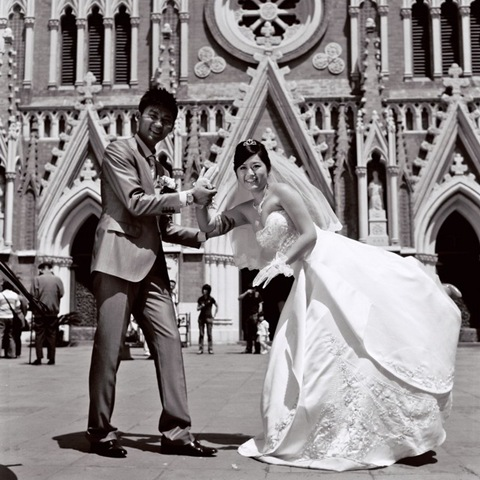
\includegraphics[scale=0.6]{wedding.jpg}
  \bicaption[fig:wedding]{婚礼}{婚礼}{Fig.}{Wedding}
\end{figure}

\begin{lstlisting}
  \begin{figure}[htbp]
    \centering
    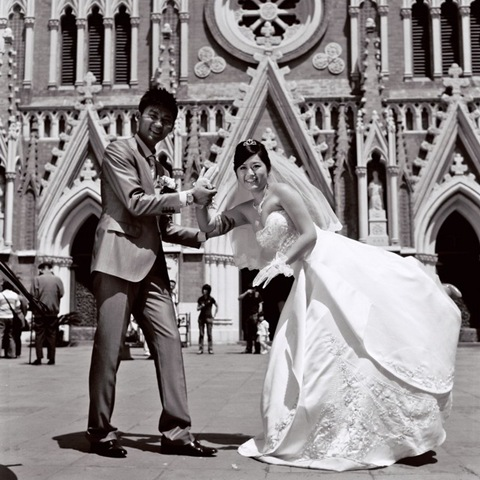
\includegraphics[scale=0.6]{wedding.jpg}
    \bicaption[fig:wedding]{婚礼}{婚礼}{Fig.}{Wedding}
  \end{figure}
\end{lstlisting}

\texttt{includegraphics}的基本参数见表~\ref{tab:figure}。

\begin{table}[htbp]
  \centering
  \bicaption[tab:figure]{插图命令参数}{插图命令参数}{Tab.}{Parameter}
  \vspace{0.2cm}
  \wuhao
  \begin{tabularx}{0.8\textwidth{}}{lX}
    \toprule
    参数             & 说明 \\
    \midrule
    width=x,height=y & 宽度和高度,绝对尺寸,可用任意长度单位。  \\
    scale=s          & 缩放比。绝对尺寸和缩放比用一种即可,同时使用两者,绝对尺寸起作用。 \\
    keepaspectratio & 保持图形比例。宽度和高度通常设置一个即可,否则图形比
    例会失调,除非再加上此选 项,
    这样图形宽度和高度都不超过指定参数。     \\
    angle=a          & 逆时针旋转角度,单位是度。  \\
    \bottomrule
  \end{tabularx}
\end{table}

对于图~\ref{fig:wedding},只使用了\texttt{scale}这一个参数,缩放因子是0.6。
当然,也可以直接指定图形的宽度和高度。图~\ref{fig:sun}的源代码如下:

\begin{lstlisting}
  \begin{figure}[htbp]
    \centering
    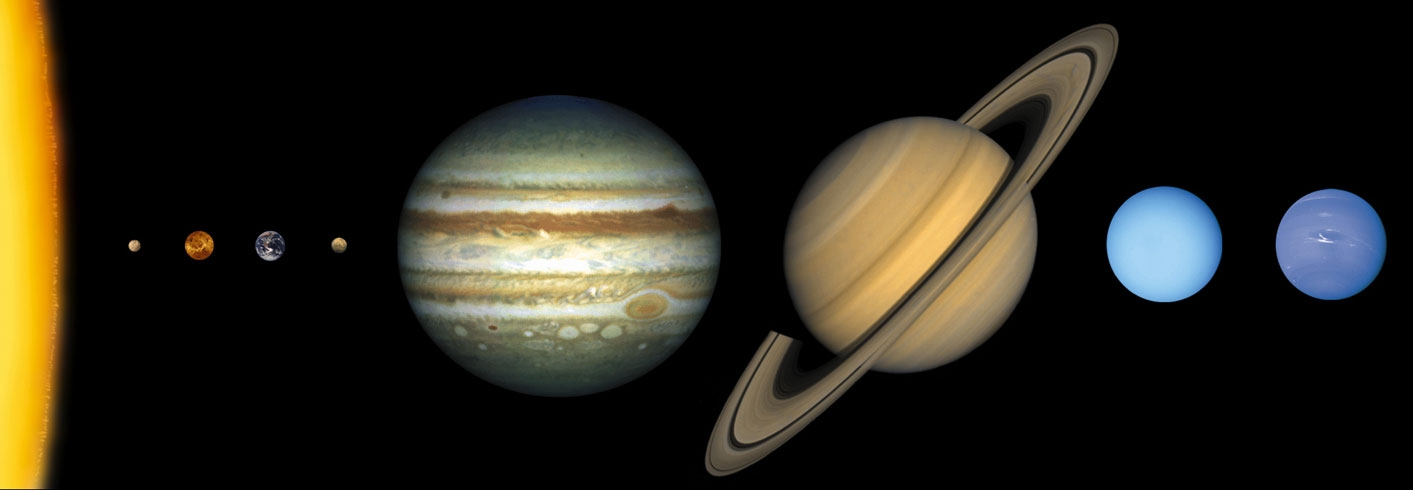
\includegraphics[width=\textwidth{},keepaspectratio]{sun.jpg}
    \bicaption[fig:sun]{太阳系}{最左侧是太阳,向右依序为水星、金
      星}{Fig.}{Outward from the Sun, the planets are Mercury, Venus,
      Earth, Mars, Jupiter, Saturn, Uranus and Neptune.}
  \end{figure}
\end{lstlisting}

可以看到,图~\ref{fig:sun}的宽度指定为版芯的宽度,然后使用了保持宽高比这
个选项。

\begin{figure}[tbph]
\usetikzlibrary{calc,through}
  \centering
    \begin{tikzpicture}
    \coordinate [label=left:$A$] (A) at (0,0);
    \coordinate [label=right:$B$] (B) at (0.75,0.25);
    \coordinate [label=above:$C$] (C) at (1,1.5);
    \draw (A) -- (B) -- (C);
    \coordinate [label=above:$D$] (D) at
    ($ (A) ! .5 ! (B) ! {sin(60)*2} ! 90:(B) $) {};
    \node (H) [label=135:$H$,draw,circle through=(C)] at (B) {};
    \draw (D) -- ($ (D) ! 3.5 ! (B) $) coordinate [label=below:$F$] (F);
    \draw (D) -- ($ (D) ! 2.5 ! (A) $) coordinate [label=below:$E$] (E);
    \end{tikzpicture}

    \bicaption[fig:sun]
    {长标题示例}
    {一个很长很长很长很长很长很长很长很长很长很长很长很长很长很长很长的标题示例
    这个图形是由Tikz绘制当然你也可以用JPG图片}
    {Fig.}
    {a long long long long long long long long long long long long caption}
\end{figure}

\begin{lstlisting}
    \begin{figure}[tbph]
        \usetikzlibrary{calc,through}
        \centering
        \begin{tikzpicture}
            \coordinate [label=left:$A$] (A) at (0,0);
            \coordinate [label=right:$B$] (B) at (0.75,0.25);
            \coordinate [label=above:$C$] (C) at (1,1.5);
            \draw (A) -- (B) -- (C);
            \coordinate [label=above:$D$] (D) at
            ($ (A) ! .5 ! (B) ! {sin(60)*2} ! 90:(B) $) {};
            \node (H) [label=135:$H$,draw,circle through=(C)] at (B) {};
            \draw (D) -- ($ (D) ! 3.5 ! (B) $) coordinate [label=below:$F$] (F);
            \draw (D) -- ($ (D) ! 2.5 ! (A) $) coordinate [label=below:$E$] (E);
        \end{tikzpicture}

        \bicaption[fig:sun]
        {长标题示例}
        {一个很长很长很长很长很长很长很长很长很长很长很长很长很长很长很长
        的标题示例这个图形是由TikZ绘制当然你也可以用JPG图片}
        {Fig.}
        {a long long long long long long long long long long long long caption}
    \end{figure}
\end{lstlisting}

长图题一般没有必要在插图目录中也完整显示,可使用菜单\texttt{Insert -{}-\textgreater{} Short
Title} 插入短标题 \verb|\index{ct\@插图\!dbt\@ 短标题} |。模板中已将图表编号两边设置了小的间距,不必再手动加入空格。


\section{双图并列}[Two Figures]

并列图示例如图\ref{fig:lang}与图\ref{fig:niang}所示。

\begin{figure}[htbp]
  \centering
  \begin{minipage}{0.4\textwidth}
    \centering
    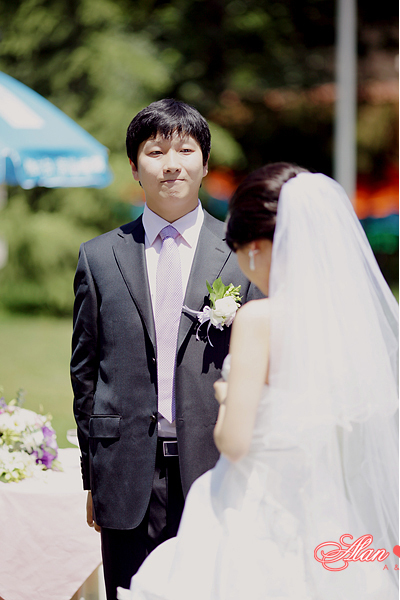
\includegraphics[keepaspectratio]{lang.jpg}
    \bicaption[fig:lang]{新郎}{新郎}{Fig.}{Bridegroom}
  \end{minipage}
  \begin{minipage}{0.4\textwidth}
    \centering
    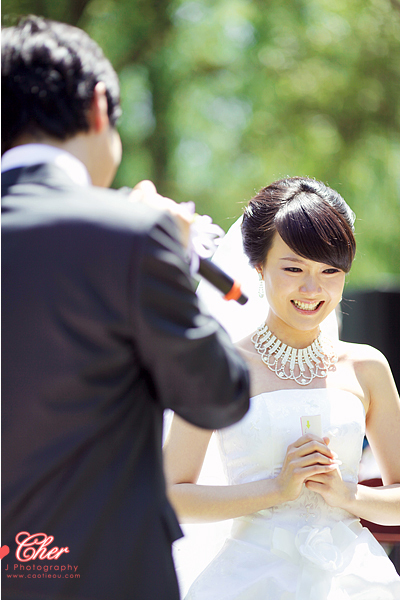
\includegraphics[keepaspectratio]{niang.jpg}
    \bicaption[fig:niang]{新娘}{新娘}{Fig.}{Brige}
  \end{minipage}
\end{figure}

\begin{lstlisting}
  \begin{figure}[htbp]
    \centering
    \begin{minipage}{0.4\textwidth}
      \centering
      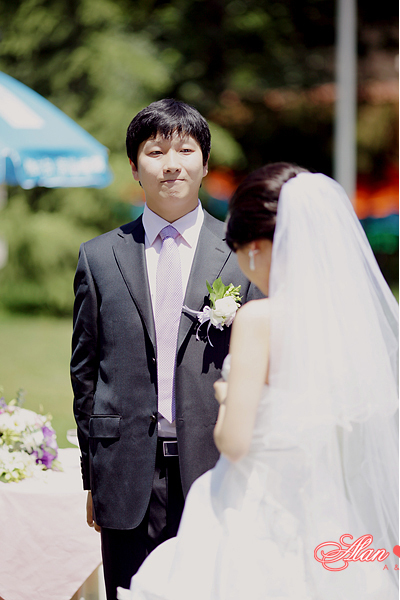
\includegraphics[keepaspectratio]{lang.jpg}
      \bicaption[fig:lang]{新郎}{新郎}{Fig.}{Bridegroom}
    \end{minipage}
    \begin{minipage}{0.4\textwidth}
      \centering
      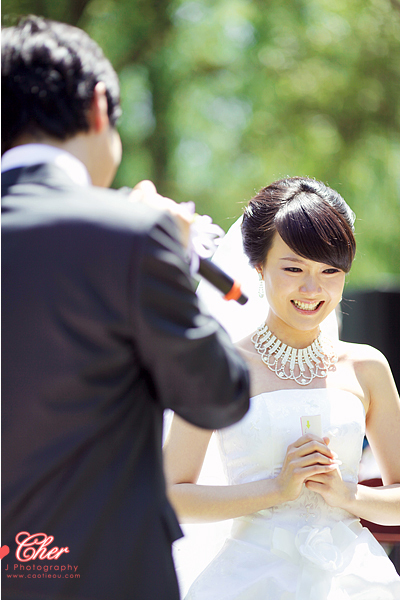
\includegraphics[keepaspectratio]{niang.jpg}
      \bicaption[fig:niang]{新娘}{新娘}{Fig.}{Brige}
    \end{minipage}
  \end{figure}
\end{lstlisting}

如果想要两幅并排的插图各有自己的标题,可以在 figure 环境中使用两
个 minipage 环境,每个里面插入一幅图 (见图~\ref{fig:lang}和
图~\ref{fig:niang}) 。不用 minipage 的话,因为插图标题的缺省宽度是
整个行宽,两幅插图就会上下排列。

这里指定了每个 minipage 的宽度为0.4倍的版芯宽度。当然,也可以自
己指定,只是两个宽度加起来不超过版芯宽度就可以了。

\section{两子图并列}[Sub Figure]

子图并列示例如图\ref{fig:judy}所示。

\begin{figure}[htbp]
    \centering
    \subfigure{\label{{fig:1a}}}\addtocounter{subfigure}{-2}
    \subfigure[Girl A]{\subfigure[女孩A]{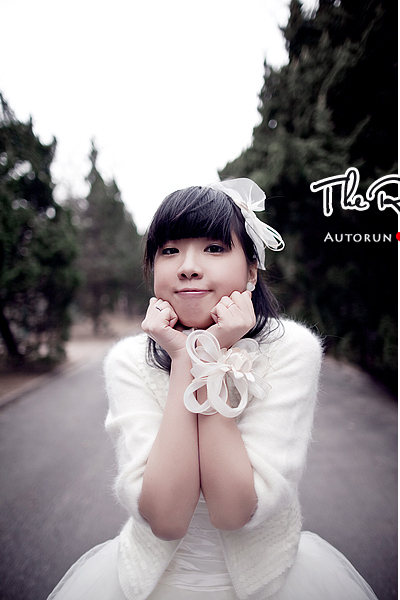
\includegraphics[keepaspectratio]{chao.jpg}}}
    \hspace{20pt}
    \subfigure{\label{{fig:1b}}}\addtocounter{subfigure}{-2}
    \subfigure[Girl B]{\subfigure[女孩B]{
\includegraphics[keepaspectratio]{ren.jpg}}}
    \bicaption[fig:judy]{女孩}{女孩}{Fig.}{Judy}
\end{figure}

\begin{lstlisting}
  \begin{figure}[htbp]
    \centering
    \subfigure{\label{{fig:1a}}}\addtocounter{subfigure}{-2}
    \subfigure[Girl A]{\subfigure[女孩A]{
        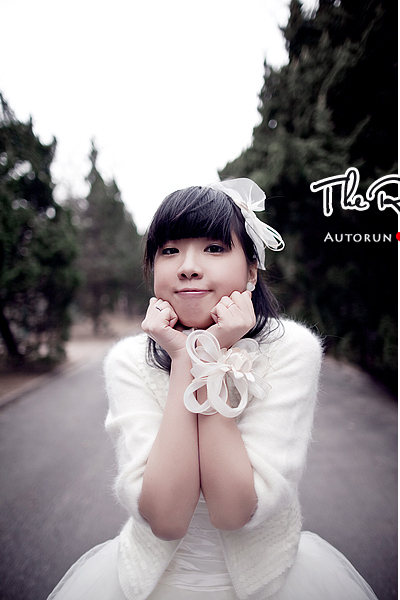
\includegraphics[keepaspectratio]{chao.jpg}}
    }
    \hspace{20pt}
    \subfigure{\label{{fig:1b}}}\addtocounter{subfigure}{-2}
    \subfigure[Girl B]{\subfigure[女孩B]{
        
\includegraphics[keepaspectratio]{ren.jpg}}
    }
    \bicaption[fig:judy]{女孩}{女孩}{Fig.}{Judy}
  \end{figure}
\end{lstlisting}


如果想要两幅并排的图片共享一个标题,并且各有自己的子标题,学位论文规范要求不止总图的标题为中英文形式,其各个子图也应具有中英文形式的标题。
然而~ccaption~宏包却无法实现子图的中英文标题功能,这里采用对 \verb|\subfigure| 命令进行嵌套的方法来实现子图的中英文标题功能。如图~\ref{fig:judy},子图的标题用命令 \verb|\subcaption| 即可。
学位论文规范要求不止总图的标题为中英文形式,其各个子图也应具有中英文形式的标题。
然而~ccaption~宏包却无法实现子图的中英文标题功能,这里采用对 \verb|\subfigure| 命令进行嵌套的方法来实现子图的中英文标题功能。


\section{pgf/TikZ~插图}[pgf/TikZ Figure]
pgf/TikZ是一个在tex系统中的画图宏包,除了可以精确的作图外,对于某些不要求精确控制的图形绘制,如:流程图,树图,等等,也提供了简便易用的支持。
下面这张图片是用TikZ宏包进行绘制的图形,其实现代码为:
\begin{lstlisting}
    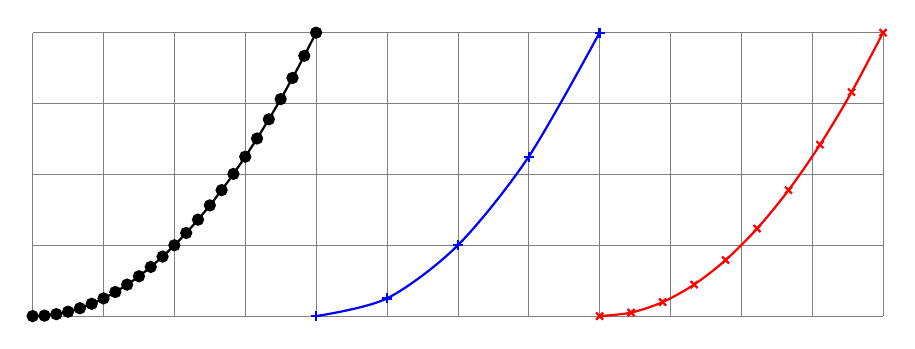
\begin{tikzpicture}[thick,smooth,domain=0:4,scale=0.9]
        \draw[very thin,gray] (0,0) grid (12,4);
        \draw plot[mark=*] (\x,{\x * \x/4});
        \draw[blue,xshift=4cm] plot[samples=5,mark=+] (\x,{\x * \x/4});
        \draw[red,xshift=8cm] plot[samples=10,mark=x] (\x,{\x * \x/4});
    \end{tikzpicture}
\end{lstlisting}

\begin{figure}[htbp]
    \centering
    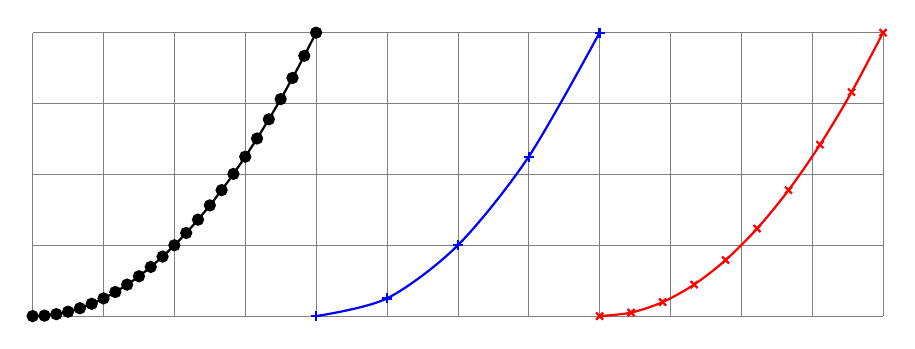
\begin{tikzpicture}[thick,smooth,domain=0:4,scale=0.9]
        \draw[very thin,gray] (0,0) grid (12,4);
        \draw plot[mark=*] (\x,{\x * \x/4});
        \draw[blue,xshift=4cm] plot[samples=5,mark=+] (\x,{\x * \x/4});
        \draw[red,xshift=8cm] plot[samples=10,mark=x] (\x,{\x * \x/4});
    \end{tikzpicture}
  \bicaption[fig:TikZ]{TikZ插图}{TikZ插图}{Fig.}{Draw with TikZ}
\end{figure}

使用pgf/TikZ可以直接使用数据表绘图,如图~\ref{fig:TikZTable},其实现代码和数据如下。

\wuhao{
\begin{lstlisting}
\begin{figure}[htbp]
    \centering
	\begin{tikzpicture}[scale=0.85]
	\pgfplotstableread{
	budget    name1   name2   name3   name4    name5    name6
	0.2 1   1   1   1   1   1
	0.4 10  10  10  10  10  10
	0.6 30  30  30  30  30  30 
	0.8 50  49  51  48  50  50
	1.0 110 110 110 110 110 110
	1.2 120 110 120 110 110 110
	1.4 130 130 130 110 110 130
	1.6 150 150 150 110 110 150
	1.8 160 150 150 160 111 150
	2.0 170 170 170 100 160 160
	}{\datatable}
	\begin{axis}[
	    width = \linewidth, height = 0.5\linewidth,
	    title style={at={(0.5,-0.35)}},
	    xtick pos=bottom,
	    ytick pos=left,
	    ybar=0,
	    ylabel={ylabel},
	    ylabel style={at={(axis description cs:0.03,0.5)}},
	    ytick={0,20,...,180},
	    bar width=4pt, ymin=0, ymax=180,
	    legend image code/.code={\draw [#1] (0cm,-0.1cm) rectangle (0.35cm,0.1cm);
	    },
	    legend style={
	        legend pos=north west,
	        nodes={scale=1},
	        draw = none,
	        cells={anchor=west}, 
	    },
	    xlabel={xlabel},
	    xtick=data,
	    xticklabels from table={\datatable}{budget},
	    ]
	
	\newcommand{\mysubplot}[2]{
	    \addplot[#2] table [x=budget,y=#1] {\datatable};
	    \addlegendentry{#1};
	}
	\mysubplot{name1}{}
	\mysubplot{name2}{pattern=crosshatch dots}
	\mysubplot{name3}{pattern=north east lines}
	\mysubplot{name4}{pattern=crosshatch}
	\mysubplot{name5}{pattern=north west lines}
	\mysubplot{name6}{fill=black}
	
	\end{axis}
	\end{tikzpicture}
   \bicaption[fig:TikZTable]{TikZ数据表绘图}{TikZ数据表}{Fig.}{Draw with Data Table}
\end{figure}
\end{lstlisting}
}

\begin{figure}[htbp]
    \centering
	\begin{tikzpicture}[scale=0.85]
	\pgfplotstableread{
	budget    name1   name2   name3   name4    name5    name6
	0.2 1   1   1   1   1   1
	0.4 10  10  10  10  10  10
	0.6 30  30  30  30  30  30 
	0.8 50  49  51  48  50  50
	1.0 110 110 110 110 110 110
	1.2 120 110 120 110 110 110
	1.4 130 130 130 110 110 130
	1.6 150 150 150 110 110 150
	1.8 160 150 150 160 111 150
	2.0 170 170 170 100 160 160
	}{\datatable}
	\begin{axis}[
	    width = \linewidth, height = 0.5\linewidth,
	    %title={The Title},
	    title style={at={(0.5,-0.35)}},
	    xtick pos=bottom,
	    ytick pos=left, % remove the tick from the right and top
	    ybar=0,
	    ylabel={ylabel},
	    ylabel style={at={(axis description cs:0.03,0.5)}},
	    ytick={0,20,...,180},
	    bar width=4pt,
	    %enlarge x limits=0.15,
	    ymin=0, ymax=180,
	    % legned related -------------
	    legend image code/.code={
	        \draw [#1] (0cm,-0.1cm) rectangle (0.35cm,0.1cm);
	    },
	    legend style={
	        %at={(0.13,1)},
	        legend pos=north west,
	        nodes={scale=1},
	        draw = none,        % without box
	        cells={anchor=west}, % algin left
	    },
	    xlabel={xlabel},
	    % xtick related 
	    xtick=data,
	    xticklabels from table={\datatable}{budget},
	    %xticklabel style={
	    %j    rotate=45,xshift=-100,yshift=-100,anchor=mid east
	    %j},
	    ] % end of options of axis environment
	
	\newcommand{\mysubplot}[2]{
	    \addplot[#2] table [x=budget,y=#1] {\datatable};
	    \addlegendentry{#1};
	}
	\mysubplot{name1}{}
	\mysubplot{name2}{pattern=crosshatch dots}
	\mysubplot{name3}{pattern=north east lines}
	\mysubplot{name4}{pattern=crosshatch}
	\mysubplot{name5}{pattern=north west lines}
	\mysubplot{name6}{fill=black}
	
	\end{axis}
	\end{tikzpicture}
   \bicaption[fig:TikZTable]{TikZ数据表绘图}{TikZ数据表}{Fig.}{Draw with Data Table}
\end{figure}

pgf/TikZ不仅可以使用文档内部数据绘图,还可以直接读取外部~csv~数据文件进行绘图,如图 ~\ref{fig:TikZcsv}~便是
读取~\texttt{data/datafile1.csv}~数据文件完成的绘图。

\wuhao{
\begin{lstlisting}
\begin{figure}[htbp]
    \centering
 \begin{tikzpicture}[scale=0.85]
    \pgfplotstableread{data/datafile1.csv}{\datatable}
    \begin{axis}[
        xlabel={Computation time passed~[minutes]},
        ylabel={bits per channel use},
        ylabel style={at={(axis description cs:0.06,0.5)}},
        xmin= 0, xmax= 120, ymin= 0,
        legend style = {
            legend pos=south east,
            legend columns = {2},
            nodes={scale=0.5}, 
        },
        grid = major,
        grid style=dashed,
        mark repeat={8},
        width = \linewidth,
        height = 0.5\linewidth,
        mark options={solid},
        every axis/.append style={
            extra description/.code={
                \node[scale=0.5] at (0.07,0.93) {Information Rate};
                \node[scale=0.5] at (0.93,0.93) {Information Rate};
            },
        },
    ]

    \addplot[red,mark=o,dashed] table [x index=0, y index=1] {\datatable};
    \addlegendentry{EM-type algorithm~[13] with 4-state FSMC}
    \addplot[dashed,mark=o] table [x index=0, y index=2] {\datatable};
    \addlegendentry{EM-type algorithm~[13] with 16-state FSMC}
    \addplot[blue,mark=diamond] table [x index=0, y index=3] {\datatable};
    \addlegendentry{Algorithm~11 with 1-qubit QSC}
    \addplot[red,mark=+] table [x index=0, y index=4] {\datatable};
    \addlegendentry{Algorithm~11 with 4-state FSMC}
    \addplot[mark=+] table [x index=0, y index=5] {\datatable};
    \addlegendentry{Algorithm~11 with 16-state FSMC}
    \addplot[red,mark=diamond] table [x index=0, y index=6] {\datatable};
    \addlegendentry{Algorithm~11 with 2-qubit QSC}
    \addplot[dashed] table [x index=0, y index=7] {\datatable};
    \addlegendentry{Estimated Information Rate~(Alg.~9)}

    \end{axis}
    \end{tikzpicture}
   \bicaption[fig:TikZcsv]{TikZ数据文件绘图}{TikZ数据文件绘图}{Fig.}{Draw with Data File}
\end{figure}
\end{lstlisting}
}

\begin{figure}[htbp]
    \centering
 \begin{tikzpicture}[scale=0.85]
    \pgfplotstableread{data/datafile1.csv}{\datatable}
    \begin{axis}[
        xlabel={Computation time passed~[minutes]},
        ylabel={bits per channel use},
        ylabel style={at={(axis description cs:0.06,0.5)}},
        xmin= 0, xmax= 120, ymin= 0,
        legend style = {
            legend pos=south east,
            legend columns = {2},
            nodes={scale=0.5}, % make the legend box smaller
            %font = {\tiny},
        },
        grid = major,
        grid style=dashed,
        mark repeat={8},
        width = \linewidth,
        height = 0.5\linewidth,
        mark options={solid},
        %% extra label for information rate
        every axis/.append style={
            extra description/.code={
                \node[scale=0.5] at (0.07,0.93) {Information Rate};
                \node[scale=0.5] at (0.93,0.93) {Information Rate};
            },
        },
    ]

    %1
    \addplot[red,mark=o,dashed] table [x index=0, y index=1] {\datatable};
    \addlegendentry{EM-type algorithm~[13] with 4-state FSMC}
    %2
    \addplot[dashed,mark=o] table [x index=0, y index=2] {\datatable};
    \addlegendentry{EM-type algorithm~[13] with 16-state FSMC}
    %3
    \addplot[blue,mark=diamond] table [x index=0, y index=3] {\datatable};
    \addlegendentry{Algorithm~11 with 1-qubit QSC}
    %4
    \addplot[red,mark=+] table [x index=0, y index=4] {\datatable};
    \addlegendentry{Algorithm~11 with 4-state FSMC}
    %5
    \addplot[mark=+] table [x index=0, y index=5] {\datatable};
    \addlegendentry{Algorithm~11 with 16-state FSMC}
    %6
    \addplot[red,mark=diamond] table [x index=0, y index=6] {\datatable};
    \addlegendentry{Algorithm~11 with 2-qubit QSC}
    %7
    \addplot[dashed] table [x index=0, y index=7] {\datatable};
    \addlegendentry{Estimated Information Rate~(Alg.~9)}

    \end{axis}
    \end{tikzpicture}
   \bicaption[fig:TikZcsv]{TikZ数据文件绘图}{TikZ数据文件绘图}{Fig.}{Draw with Data File}
\end{figure}
   
更多的关于pgf/TikZ绘图方法请参考相关资料。

\section*{本章小结}[Brief Summary]
插图方法介绍。
